\documentclass[handout]{beamer}

\usepackage[french]{babel}
\usepackage[utf8]{inputenc}
\usepackage{listings}
\usetheme{CambridgeUS}

\title{JBoss AS 101}
\subtitle{JBoss Basic Usage}

\author{Romain PELISSE}
\institute{ESME Sudria}
\date{\today}

\logo{
\includegraphics[scale=0.3]{../img/logo-cc.png}}

\begin{document}
	% Definition de l'affichage de l'ensemble des codes
	\definecolor{white}{rgb}{1,1,1}
	\definecolor{vert_commentaire}{rgb}{0.03, 0.45, 0}
	\definecolor{rouge_chaine}{rgb}{0.128, 0, 0}
	% Définition du langage Ant
	\lstdefinelanguage{ant}
	{
		morekeywords={name,default,basedir,value,property,depends},
		otherkeywords={<project,</project>,<target,/target>,<echo>,</echo>},
		sensitive=false,
		morecomment=[s]{<!--}{-->},
		morecomment=[s]{<?xml}{?>},
		morestring=[b][\color{red}]",
	}

	\lstset{
		language=ant, 
		backgroundcolor=\color{white}, 
		basicstyle=\small, 
		showstringspaces=false,
		stringstyle=\ttfamily,
		commentstyle=\color{vert_commentaire},
		keywordstyle=\color{blue}\bfseries\emph
	}

% end...
\frame{\titlepage}

\section[Outline]{}
\frame{\tableofcontents}

\section{A Short JBoss history}
	\begin{frame}{EJB Open Source Software}
		\begin{block}{An Open Source, full Java, implementation of EJB Specification}
			\begin{itemize}
				\item Designed by Marc Fleury
				\item EJB Open Source Softare become JBoss AS
				\item Fleury left SUN to create JBoss Inc., professionnal support to JBoss
				\item JBoss become the first Open Source AS compliant to J2EE 
			\end{itemize}
		\end{block}
		\begin{block}{Professional Open Source}
			\begin{itemize}
				\item Open Source Software 
				\item Support 
			\end{itemize}
		\end{block}	
	\end{frame}
\section{What is JBoss AS ?}
	\begin{frame}
		\begin{block}{J2EE Specification}
			\begin{itemize}
				\item Defines an application server duties
				\item Set of technical services, most likely to required by to any application
				\begin{itemize}
					\item Security : JAAS Implementation
					\item Servlet Container (Servlet, JSP) : Tomcat Web Server
					\item JMS Implementation : JBossMQ, JBossMessaging
					\item Database access : Support for Oracle,MySQL,...
					\item Web Services : Axis,JBossWS
					\item Transactionnal monitoring : Arjuna
				\end{itemize}
			\end{itemize}
		\end{block}
		\begin{block}{Purpose of the specification}
			\begin{itemize}
				\item Basicly, J2EE specification defines what an application server should do (not how is should do it)
				\item Application development is focused on business logic
			\end{itemize}
		\end{block}

	\end{frame}
	\begin{frame}
		Application Server : An integration product
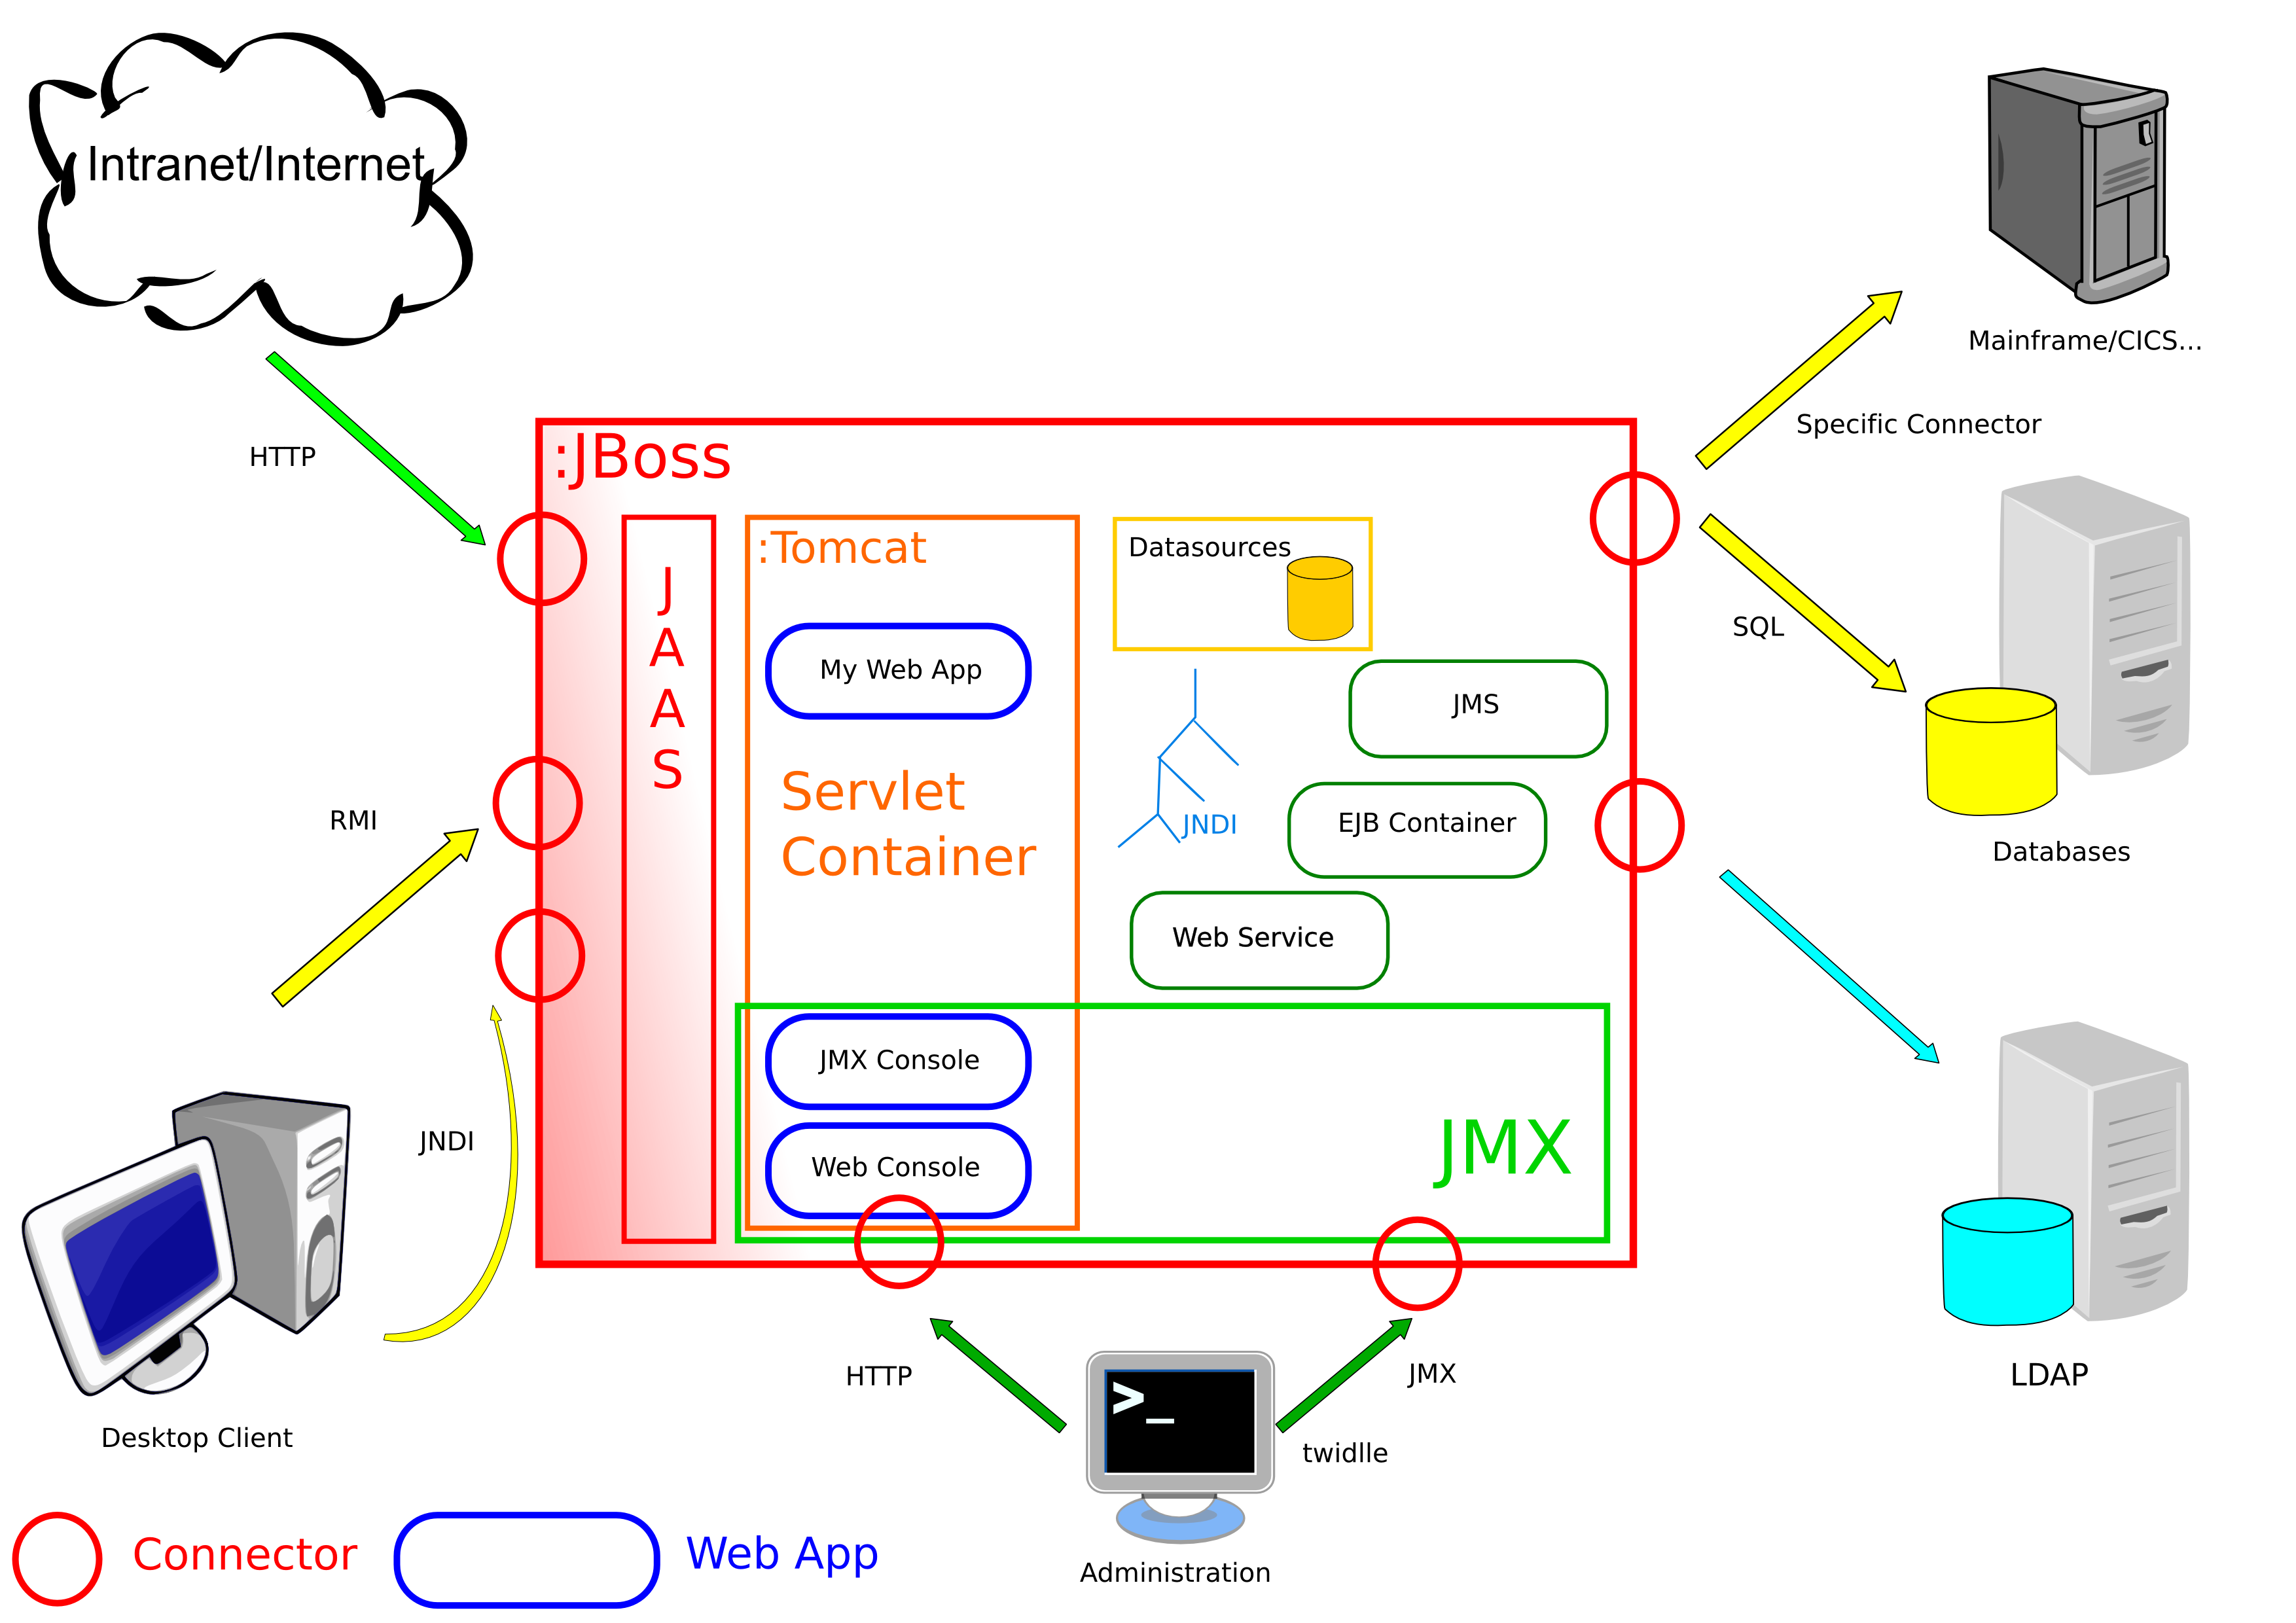
\includegraphics[scale=0.4]{../img/whatisjbossas.png}
	\end{frame}
\section{JBoss directory tree}
	\begin{frame}
		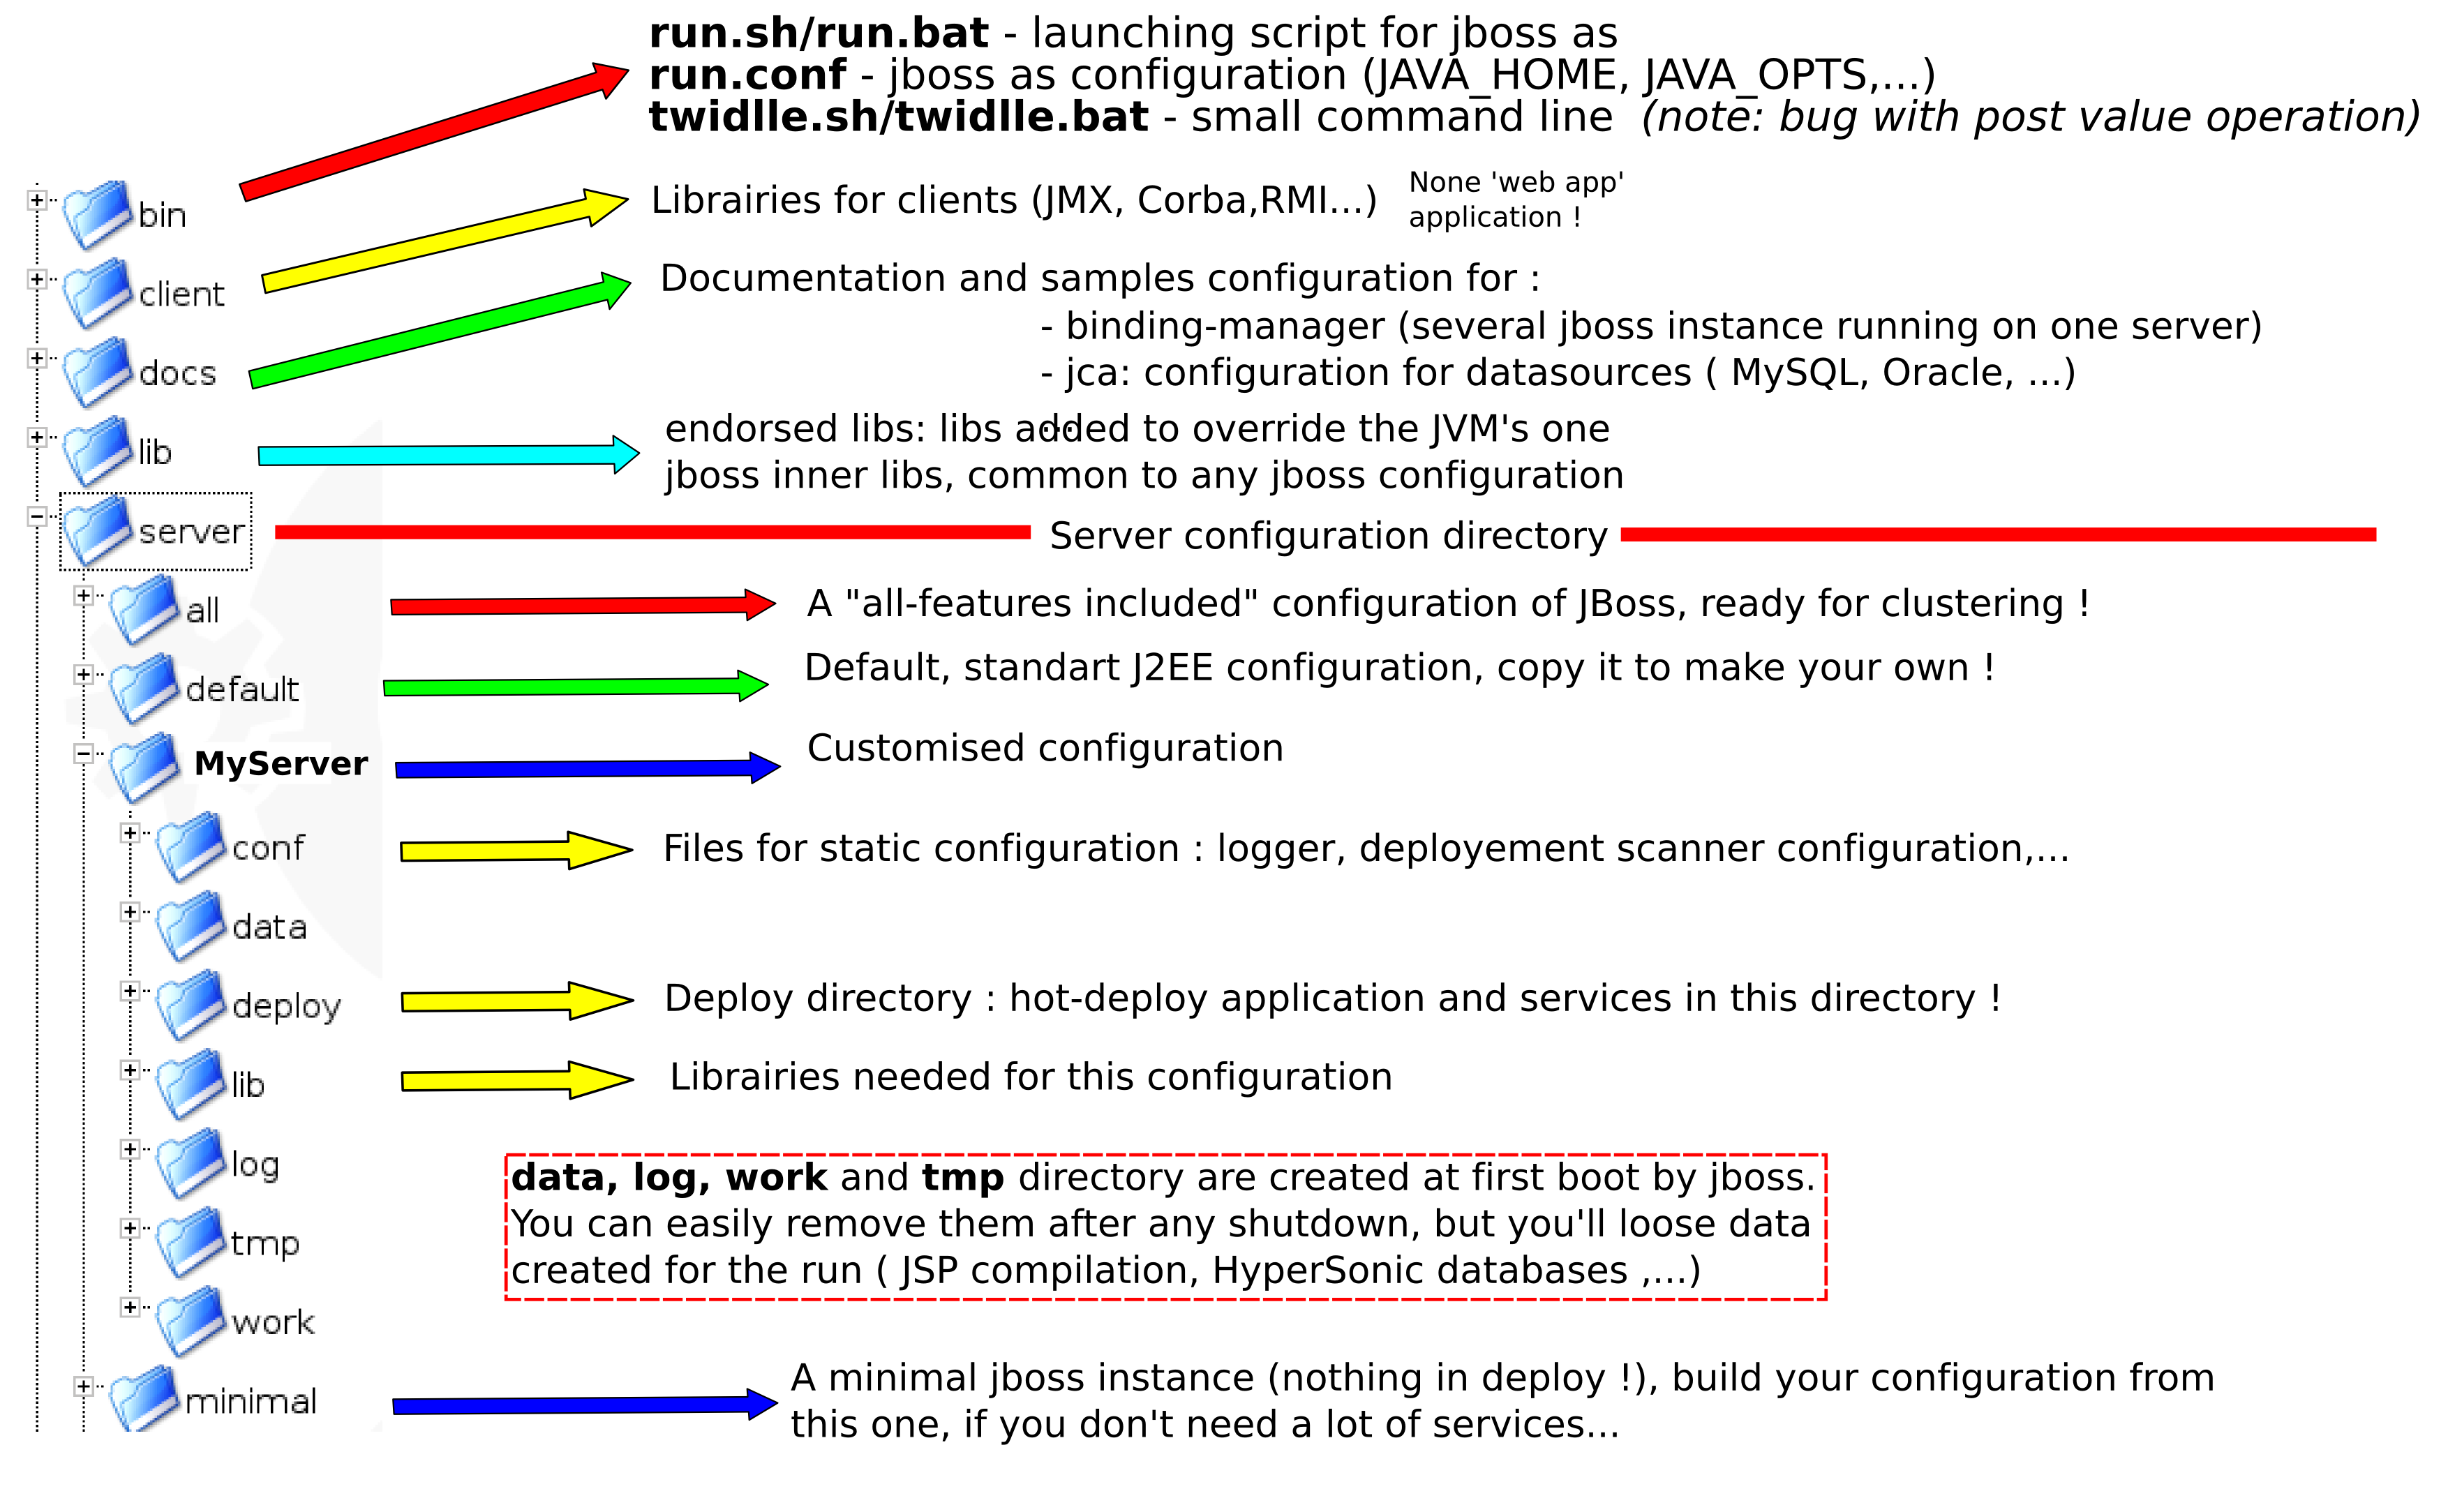
\includegraphics[scale=0.4]{../img/jbossdirectorytree.png}			 
	\end{frame}
\section{TD: Running JBoss}
	\begin{frame}
		\begin{block}{Create your configuration}
			Simply copy \textit{default} configuration into a new folder
		 	\$ cp -R default td
			Ready to run !
		\end{block}
		\begin{block}{Let's run...}
			\$\{JBOSS\_HOME\}/bin/run.sh -c td -b 127.0.0.1
			\begin{itemize}
				\item	-c : specify the configuration ( default is \textit{default} )
				\item	-b : specify IP binding ( by default binds on any interfaces )
			\end{itemize}
		\end{block}
		\begin{center}
			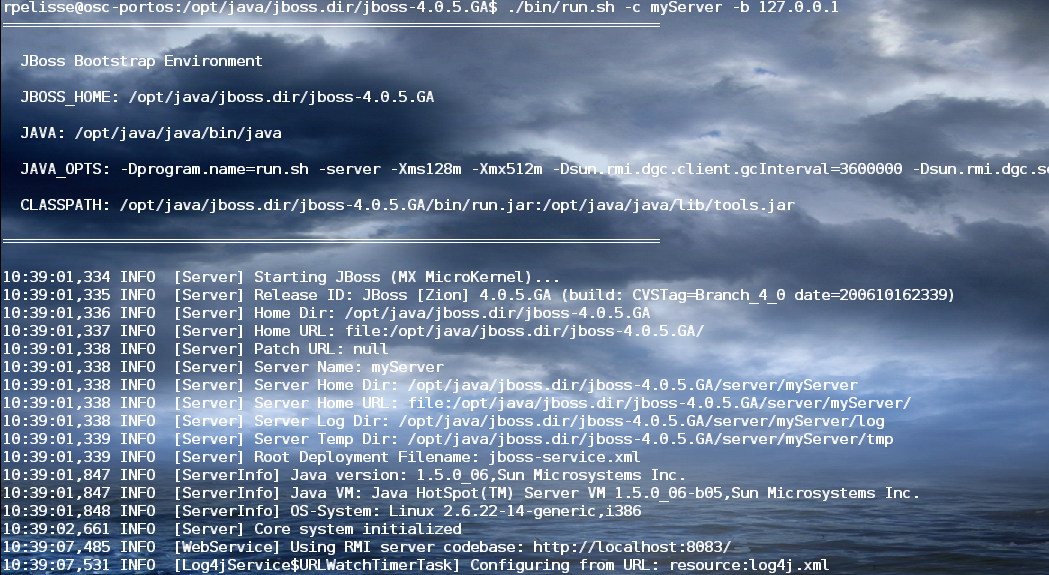
\includegraphics[scale=0.15]{../img/jboss-start.png}
		\end{center}
	\end{frame}
\section{Package and deploy application}
	\begin{frame}
	 	\begin{block}{Standart J2EE packaging format}
	 	 	J2EE application are simple directory tree (that may be zipped). Suffix indicates type of application:
			\begin{itemize}
				\item war : Web Archive, simple web application (no EJB)
				\item ear : Entreprise Archive (EJB application)
				\item sar : Service Archive (Specific to JBoss, the application is a JBoss Service)
				\item jar : Java Archive
			\end{itemize}
	 	\end{block}
	\end{frame}
	\begin{frame}
	 	\begin{block}{Deployement order}
			JBoss deploys application according to there suffix, plus some jboss-specific mecanism
			\begin{enumerate}
				\item deploy.first/, if this directory exist in deploy folder
				\item *.sar 
				\item *.ear
				\item *.war
				\item deploy.last/
			\end{enumerate}
		\end{block}
	\end{frame}
	\begin{frame}
		\begin{block}{How to deploy}
			Simply put the file/directory, with the proper suffix, into the server/\textit{config}/deploy directory to deploy it.
			\begin{itemize}
				\item Remote loading is possible (seldom used)
				\item \textbf{Russian Doll} packaging (ex: a jar containing a war and an other jar)
				\item Creates a \textbf{Classloader} per top-level deployement
			\end{itemize}
		\end{block}
	\end{frame}
\section{TD: Deploy application}
	\begin{frame}
		\begin{block}{Deploy the jboss-101-1.0.war}
		 	To deploy the application simply copy the war file into the server/myServer/deploy.
		\end{block}
		\begin{center}
			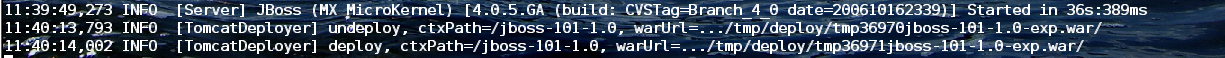
\includegraphics[scale=0.25]{../img/deploy-app.png}
		\end{center}
		\begin{block}{Deploy as a directory}
			\begin{enumerate}
				\item Remove the jboss-101-1.0.war from deploy
				\item Unzip the application into a directory named jboss-101-1.0.war/
				\item Copy the folder to \textit{deploy}
			\end{enumerate}
		\end{block}
	\end{frame}
	\begin{frame}
		\begin{block}{Remote debug in tomcat}
		 	TODO! 
		\end{block}
	\end{frame}
\section{JBoss Sliming and Tuning}
	\begin{frame}
		\begin{block}{Removing unused services}
			Services are deployed in deploy, if you don't use them, just remove them !
		 	TODO: Add url to the appropriate wiki page. 
		\end{block}
		\begin{block}{Tuning static configuration}
			Static services, such as the deployement scanner, may also be tuned, in the \textit{conf/} directory of jboss
		\end{block}
	\end{frame}
\section{TD : Tuning the server}
	\begin{frame}
		\begin{block}{Removing unused services}
			Move the deploy/jms folder to undeployed/ (create this folder), restart jboss.
			Move the deploy/hsqldb-ds.xml to undeployed/ , restart jboss
		\end{block}		
		\begin{block}{Tuning the deployement scanner}
			Edit the conf/jboss-service.xml, look for the \texttt{<mbean code="org.jboss.deployment.scanner.URLDeploymentScanner"}
			Modifying the XML code to reduce the scanner frequency and to ignore .test files.
		\end{block}		
	\end{frame}
% \section{TD : Building a conf from minimal}
% 	\begin{frame}
% 		\begin{block}{Removing unused services}
% 		\end{block}
% 	\end{frame}
\section{Port Binding}
	\begin{frame}
		\begin{block}{Removing unused services}
			\begin{itemize}
 				\item Main ports:
				\begin{itemize}
 					\item 8080 : Tomcat Web Container
					\item 1099 : JNDI
					\item ...
				\end{itemize}
				\item Connector
				\begin{itemize}
					\item HTTP
					\item AJP
				 	\item RMI (RMI over HTTP)
					\item JMX	 
				\end{itemize}
				\item Binding Manager
			\end{itemize}
		\end{block}
	\end{frame}
\section{TD: Port Binding}
	\begin{frame}
		\begin{block}{Setting up two jboss instances on the same server}
			TODO: Wiki URL
			Follow the tutorial in order to deploy a copy of your configuration
		\end{block}
	\end{frame}
% TODO:
% \section{Logging with JBoss}
% 	\begin{frame}
% 		\begin{block}{}
% 		\end{block}
% 	\end{frame}


\section{Secure access to a web application}
	\begin{frame}
	 	TODO: Add URL towards tutorial
	\end{frame}

\section{Adminstration and analysis}
	\begin{frame}
		\begin{block}{JMX Architecture}
			\begin{itemize}
			\item JBoss architecture is based on JMX specification.
			\item Any services is a Managed MBean.
			\end{itemize}
		\end{block}
		\begin{Administration tools}
		 	\item Web applications : web-console and JMX Console
			\item Command line tool : twiddle.sh/twiddle.bat
			\item Monitoring capabilities : JBoss Monitoring Services
		\end{Administration tools}
	\end{frame}
\section{TD: Administration and monitoring}
	\begin{frame}
		\begin{block}{Using JMX Console}
			Using the web app browse the jmx-console ( http://jboss-host:8080/jmx-console/ ) and find the following MBean:
Adminstration of the jboss webap
MBean Name:  	Domain Name:  	jboss.web
	type: 	Manager
	host: 	localhost
	path: 	/jboss-101-1.0

			Look to all the data you can gather on this wepapp.
		\end{block}
		\begin{block}{Using the twiddle script}
		 	Using the twiddle.sh/twiddle.bat file in the 'bin' directory
		\end{block}

	\end{frame}
\section{Clustering with JBoss}
	\begin{frame}
		\begin{block}{What is a cluster and what for ?}	
		\end{block}
	\end{frame}
\section{TD: Clustering}
	\begin{frame}
		\begin{block}{How to cluster}
		\end{block}
	\end{frame}
\end{document}